%[prl] it will mess up section numbers but puts our emails in the bibliography section
%[eqsecnum] Number equations by section
%
%
%\documentclass[prd,preprint,letterpaper]{revtex4}
\documentclass[aps,prb,twocolumn,superscriptaddress]{revtex4-1}

\usepackage{graphicx}  % this is the up-to-date package for all figures
\usepackage{amssymb}   % for math
\usepackage{verbatim}  % for the comment environment
\usepackage{color}
\usepackage{subcaption} % for subcaptions on side-by-side figures
\usepackage{float}	% allows use of 'H' command

% This allows you to use '\cref{}' to reference sections with the symbol
%\usepackage{cleveref}
%\crefname{section}{\S}{\S\S}%{§}{§§}

%\usepackage{hyperref}	% needed to add hyperlinks
%\hypersetup{
%  colorlinks=true,
%  linkcolor=blue,
%  filecolor=magenta,
%  urlcolor=cyan,
%}

\bibliographystyle{apsrev}


% these are some custom control of the page size and margins
% \topmargin= 0.2in  % these 1st two may be needed for some computers
% \textheight=8.75in
\textwidth=6.5in
%\oddsidemargin=0cm
%\evensidemargin=0cm

% this is where the actual document itself (rather than control statements) begins:

\begin{document}



\title{Assassinating ASASSN}


\author{Corey Mutnik}
\email{cmutnik@hawaii.edu}
\affiliation{Department of Physics \& Astronomy, \\
University of Hawaii at Manoa,\\
2505 Correa Rd, Honolulu, HI, 96822, USA}
\altaffiliation{ASTR 399}

% \section is used to start a new one with a heading
\begin{abstract}

\end{abstract}

\maketitle    




\section{Immediate}
\begin{itemize}
	\item{} How many cases of obs that overlap asn obj that we should have seen
	\item{} Stay within $\pm$10~days of peak night
	\item{} how many observations dont have an entry in ddt file and why
	\item{} use log files
	\item{} ~~~column 12,13 are fitted RA and Dec
	\item{} ~~~if these and magzeropoint are 0 then theres no match due to failed observation
	\item{} ~~~if ra dec mzp do exist, then it should be in the ddt file
\end{itemize}


\section{Object Cuts}

\iffalse
 ASASSN reported the discovery of 385 Supernova (SN) by October 11, 2016. \\
 100 SN have a Dec lower than -30\\
 165 SN were observed by asn before ATLAS observations began\\

 65 SN ...\\
 50/65 never had any sky/time overlap with ATLAS\\
 14/65 were 57364 or before, and the reductions were not very good\\
 1/65 (maybe) was before the SNII exploded, or it was really faint\\
 This left us with a total of 96 SN
\fi


%The primary factors restricting ATLAS observations were horizon and date.

\indent With a declination (Dec) limit of approximately $-30^{\circ}$, 100 SN were not 
%expected to show up in the ATLAS data. 
expected to be present in the ATLAS data.
%ASASSN reported another 165 SN before ATLAS was operational. 
ASASSN reported another 165 SN before ATLAS began collecting data. 
These two sets do not exist independent of one another. 
%After eliminating objects that fell below a Dec of $-30^{\circ}$ and those that 
%peaked before ATLAS was truly up and running, we were left with 161(=65+96) ASASSN SN.
After applying Dec and MJD based restrictions and accounting for overlaps between 
these groups, 161 SN remained from the initial 385 reported by ASASSN. 
%%%
Another 65 SN peaked before ATLAS was truly operational, leaving 96 as potential candidates.
%Although data was being collected, ATLAS was not instantaneously operational.
%%%
% CHECK VALIDITY OF THIS
All 96 of these objects were found in the ATLAS data, resulting in a 100\% completion rate.
%All 96 of these objects were found in the ATLAS data, giving a 100\% completion rate.
~[CHECK VALIDITY OF THIS]
%%%



%50/65 never had any sky/time overlap with ATLAS
%14/65 were 57364 or before, and the reductions were not very good
%1/65 (maybe) was before the SNII exploded, or it was really faint
%~[...]Another 65 SN peaked before ATLAS was truly operational.
\indent The 65 SN that peaked before ATLAS was truly operational can be further broken down as follows.\\
%Of these 65, 14 were reported to peak by 57364. 
%14 SN were reported to peak by 57364;
%14 SN were reported to peak on or before 57364; time during which reduced 
%ATLAS data is considered unreliable.
Reported peak brightnesses occurring on or before 57364 accounts for 14 SN. 
During this time the ATLAS reduction process was still being refined, making 
any reduced data unreliable.
%Reduction of data, by the ATLAS pipeline, was unreliable before this date.
%Data reduced by the ATLAS pipeline was not good enough to trust before 57364.
%%Another 50 fell in regions that had no overlap, due to ATLAS observations patterns.
Another 50 SN fell in regions that had no overlap with ATLAS observations due 
to the pattern in which data was collected.
%Based on observation patterns, another 50 SN are not expected to have any overlap / to have been observed.
The final case was a Type II supernova (SNII).
%The final SN was a Type II. 
%SNII are notoriously short lived. This makes it likely that...
SNII are notoriously short lived; making it likely that ATLAS observed this region of the sky in the 
time surrounding the explosion, but not during the event.
%Due to the short nature of Type II events, it is likely ATLAS observed that region of the sky in the 
%time surrounding the explosion, but not during the event.



\section{Write it all down}
\begin{itemize}
	\item{} does ddt file exist
	\item{} does ddt exist but line isnt there
	\item{} ~~~use script we previously made but {\bf record and quantify results}
\end{itemize}


\subsection{general cases [integrate sections]}
We expect to see 96 of the ASASSN SN in ATLAS observations. 
This presents us with 850 overlap opportunities, using a $\pm10~day$ window.

For the 96 SN that overlap in time and location, 850 total ATLAS 
observations are expected.
A collective 694 observations were recorded and properly reduced. 

% rephrase
No ddt files exist for any observations in the nights any single ddt 
wasn't generated; accounting for 15/850.

For 67 of the 850 possible observations, there exists a ddt file that 
lacks the correct line.

Need to better understand how diff and ddt files are created. Could it 
be pinging on negative flux (object that is dimmer since wallpaper)? 
Which requires subtraction, implied by the name difference; but, division 
is more likely.


\subsection{No ddt file}

\subsection{No diff file}

\subsection{No ddt Match}
\begin{itemize}
	\item{} ~[A] 3 is at the edge and fuzzy, causing ATLAS to miss it
	\item{} ~[B] 26 Objects are in reduced image but not in difference image.
	\item{} ~[C] 3 Object fell on a portion of the image that wasn't differenced properly and is a white chunk.
	\item{} ~[D] 17 set of fits/diff images contains nothing at the indicated x,y coordinates
	\item{} ~[E] 6 bright host galaxy, faint in difference image...must have been missed by ATLAS during difference photometry
	\item{} ~[F] 3 unusable reduced and differenced data
	\item{} ~[G] 8 unusable differenced data
	\item{} ~[H] 1 not on image
\end{itemize}

%Of the 67 occurrences missing a line in the ddt file:
%1 is at the edge and fuzzy, causing ATLAS to miss it
%x Objects are in reduced image but not in difference image. 
%Either the something was calculated incorrectly, or this isn't a transient.

Of the total 850 expected matches, 67 do not show up in existing ddt files. 

Nature constantly plays a role, when collecting astronomical data. When 
observations are made at the beginning or end of a night, ambient light 
levels rise and sky background fluctuations. [F] of the 67 missing ddt 
lines can be attributed to poor observation conditions, brought on by 
clouds and increased levels of sky background.

Errors during the image differencing process led to the loss of [G] 
expected overlaps. Older differencing techniques caused entire portions 
of images to be lost, accounting for [C] matches. \\
%Previous differencing techniques also account for [G].

%Outdated differencing procedures caused the ATLAS pipeline to miss\\
%Outdated differencing procedures caused the ATLAS pipeline not to trigger on faint\\
The ATLAS pipeline failed to trigger on faint objects. \\
%Outdated differencing procedures lead to less consistent backgrounds,\\
Outdated differencing procedures give rise to less uniform backgrounds, \\
making it harder to distinguish between faint objects and (residual noise?). 
Bight host galaxies cause SN to become extremely faint in difference images.
%Such occurrences caused the ATLAS pipeline to miss [E] matches, during the difference photometry stage.\\
Such occurrences caused the ATLAS pipeline to miss [E] matches while preforming 
photometry on the differenced images.

%The PSF across an image can vary due to numerous reasons.\\
There are various reason why the PSF across an image may vary.
Here, the major contributers are high levels of sky background and optical 
issues inherent to the ATLAS system. 
%When gone uncorrected, such issues give rise to distortion\\
%If the proper corrections aren't made, such issues give rise to distortion\\
If not properly corrected for, such issues cause observed objects to become distorted. 
%Distortion causes sharp edges to blur, making it harder for the ATLAS pipeline to identify these objects.\\
%Distortion causes sharp edges to become fuzzy, making it harder for the ATLAS pipeline to identify these objects.\\
%Distortion can cause the sharp edges of an object to become fuzzy, causing the ATLAS pipeline not to trigger on such objects.\\
%Distortion can cause sharp edges to become fuzzy, causing the ATLAS pipeline not to trigger on such objects.\\
Distortion can cause sharp edges to become fuzzy, resulting in the ATLAS pipeline 
failing to trigger on such objects.This accounts for [A] of the missing matches.
Objects that were only in reduced images, but not in differenced images, account 
for [B] of the matches missing from the ddt files.

There were [D] cases in which the SN was not detecting in either the reduced or 
differenced image. This indicates poor photometry or that the SN explosions 
occurred outside the nominal $\pm10~day$ window.

The final match missing from the ddt files comes from an issue with the array 
dimensionality. Each image is saved as an [mxn] matrix. The software that 
determines the correspondence between x,y-pixel coordinates and the objects RA,Dec 
assumed the captured image fully extended to the edges of the [mxn] matrix. \\
(Due to the way the detectors are aligned,)?\\
the edges of some collected data are not completely filled. When the frames overlap, 
the objects lie where they are expected. Looking at isolated images show that ever 
image does not fully extend to the intended edges. For the [H] particular case, the 
image data ends above the bottom edge of the array. Although the object is expected 
to be there, it does not exist on this particular image.






%\vfill\eject
\clearpage


\section{Introduction}



\subsection{ASASSN Breakdown}
The All-Sky Automated Survey for Supernovae (ASASSN) has been\\
data collected by two 14--cm telescopes\\
one at Haleakala, the other at the LCOGT Cerro Tololo station.\\
first guy started in December 2013...second came online in July 2015.\\
these two currently cover roughly 20,000~$deg^{2}$ a night\\
%they eventually plan to survey the entire sky, every night, down to 17th mag, using 16 scopes at 4 diff sites\\
~[NEED CITATIONS FOR ALL THESE]
%\footnote{http://www.astronomy.ohio-state.edu/~assassin/index.shtml}

ASASSN data~\cite{asn_data}

\begin{figure}[H]%[h!]
  \begin{center}
\centerline{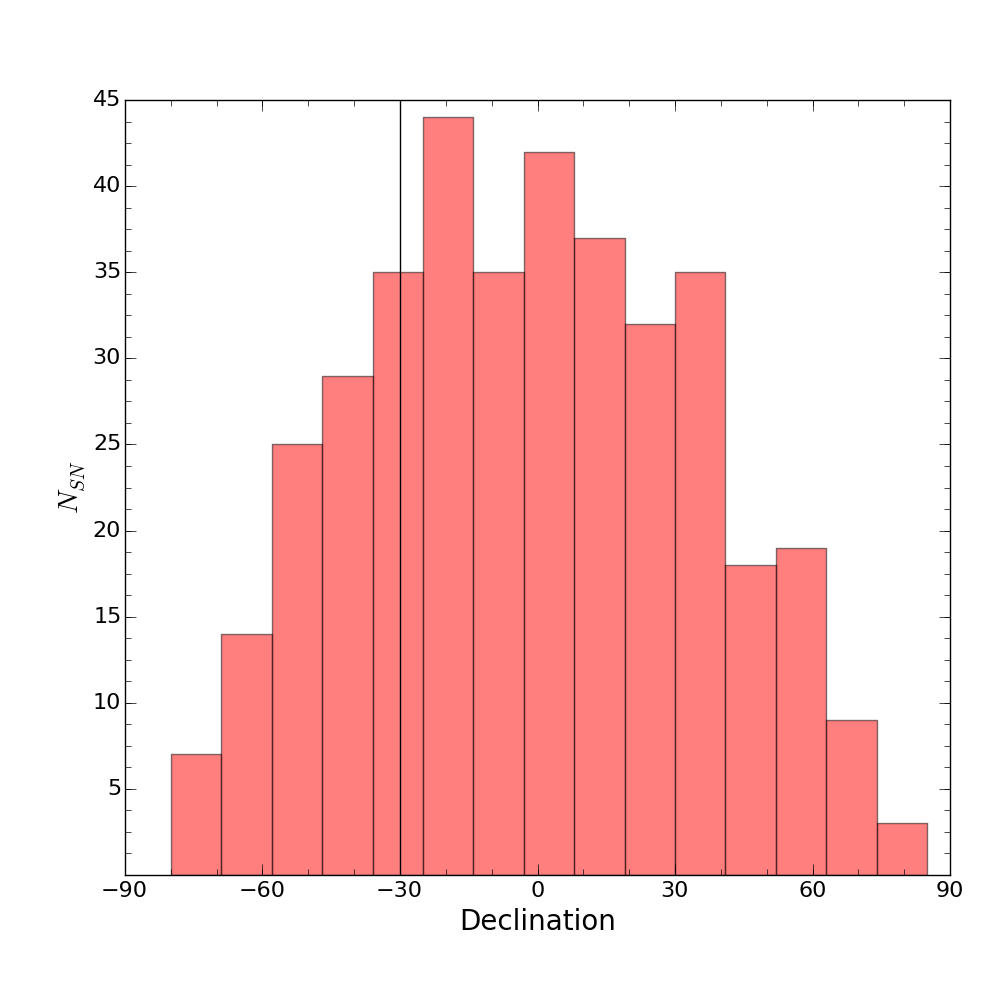
\includegraphics[width=3.35in]{figures/dec_histo_step10.png}}
\caption{\it \small{ASASSN SN sorted by their declination. The vertical line at $-30^{\circ}$ indicates the lower limit on ATLAS observations. \label{fig:asn_dec}}}
  \end{center}
\end{figure}
\begin{figure}[H]%[h!]
  \begin{center}
\centerline{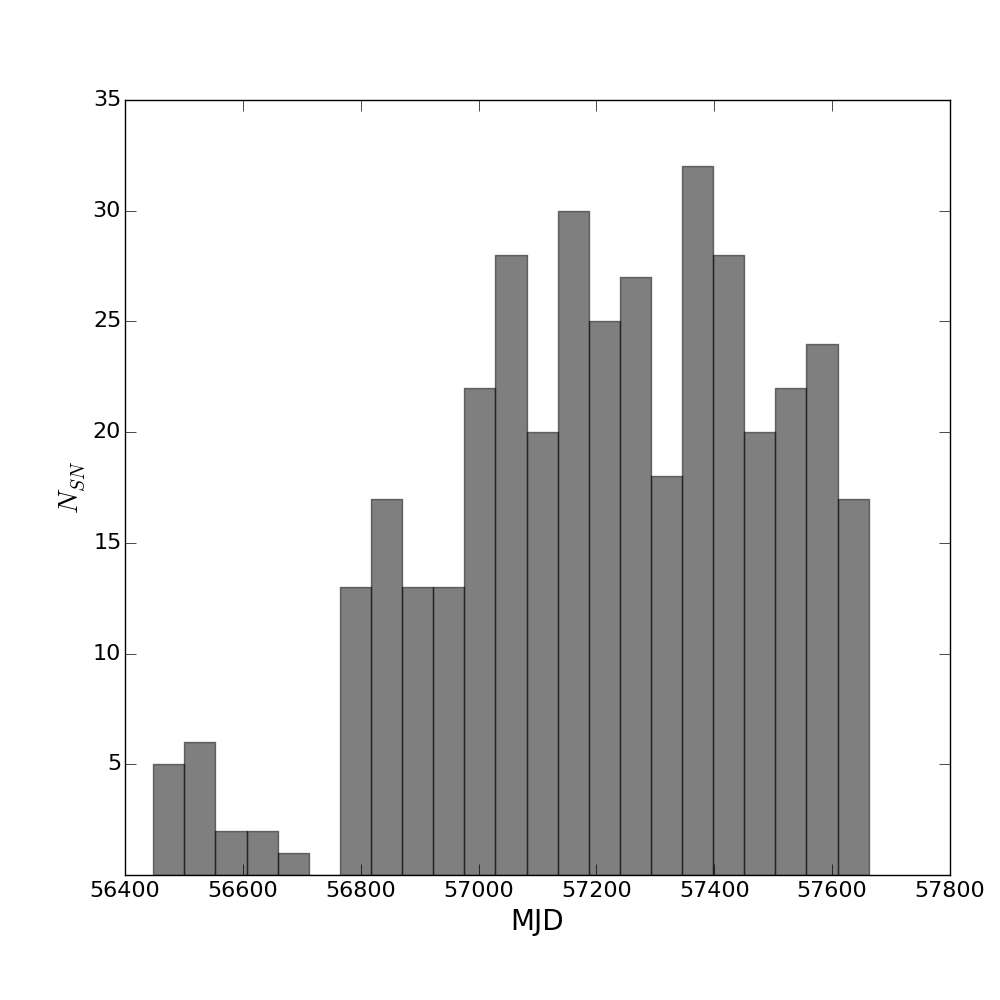
\includegraphics[width=3.35in]{figures/mjd_histo_step50.png}}
\caption{\it \small{Discovery date of ASASSN SN. \label{fig:asn_mjd}}}
  \end{center}
\end{figure}
~[MAKE THIS A DUAL FIGURE: (a) (b)]
~[REBIN MJD DATA FOR PEAK BRIGHTNESS DATE NOT DISCOVERY DATE]

\section{Goals}
Using current data collection and reduction techniques, we plan to identify SN faster and fainter than the 
ASASSN team is able to.

%\section{ATLAS PathFinder 2 Observations}
%\section{ATLAS PathFinder Data}

%\subsection{Object Cuts}\label{sec:cuts}

%\section{Conclusions}
%\section{Discussion}


\section*{Acknowledgments}
I would like to thank \input acknowledgement.tex  % input acknowledgement



\setlength{\parindent}{0cm}

\bibliography{biblio}

%\begin{thebibliography}{99}  % the trailing 99 controls some obscure format--just use
%\bibitem{Sch_eq} Weisstein, Eric W. ``Schr\"{o}dinger Equation."
%{\em Schr\"{o}dinger Equation. } Mathematica, 1996. Web. 2 May 2015.
%\end{thebibliography}

\end{document}
